\begin{comment}
  \bibliography{project.bib}
\end{comment}

\chapter{Preliminaries}
\label{cha:preliminaries}

Before we are ready to talk about loading image files, we first need
know how images are represented in a computer.

\section{RGB}
\label{sec:rgb}

There several models for representing color in a computer, but the
most prominent and popular one is by no doubt \textbf{RGB} \index{RGB}

But to understand the RGB color model, we first need to understand
color to begin with. Color is light moving at different
wavelengths. Different colors have different wavelengths. In our eyes
there are cells for perceiving three different wavelengths of light:
red, blue and green. There can also be different amounts of red, blue
and green light absorbed by the cells and the colors and also be
mixed, creating new kinds of colors. \cite{neider93:_openg_progr_guide}

\begin{figure}[h]
  \centering
  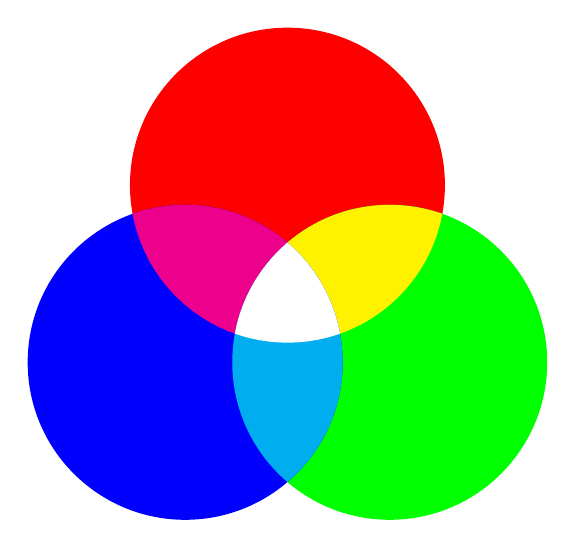
\begin{tikzpicture}

  \draw [draw=none, fill=red] (90:1.5) circle (2cm);
  \draw [draw=none, fill=green] (-30:1.5) circle (2cm);
  \draw [draw=none, fill=blue] (210:1.5) circle (2cm);

  \begin{scope}
    \clip (90:1.5) circle(2cm);
    \draw [draw=none, fill=yellow] (-30:1.5) circle (2cm);
  \end{scope}

  \begin{scope}
    \clip (210:1.5) circle(2cm);
    \draw [draw=none, fill=magenta] (90:1.5) circle (2cm);
  \end{scope}

  \begin{scope}
    \clip (-30:1.5) circle(2cm);
    \draw [draw=none, fill=cyan] (210:1.5) circle (2cm);
  \end{scope}

  \begin{scope} % red + green + blue = white
    \clip (90:1.5) circle(2cm);
    \clip (210:1.5) circle(2cm);
    \draw [draw=none, fill=white] (-30:1.5) circle (2cm);
  \end{scope}
\end{tikzpicture}
  \caption{RGB color model}
  \label{fig:rgb}
\end{figure}

So the RGB color model relies on the fact that all colors are a
mixture of red,blue and green, as it is demonstrated in figure
\ref{fig:rgb}. White is a mixture of red, blue and green, yellow is
mixture of red and green, and so on. The mixing of different amounts
of colors can conveniently enough be specified in numbers very
easily. Which brings us to:

\section{Color depth}
\label{sec:bit-depth}

\section{Digtal image}
\label{sec:digtal-image}

% Images can most easily be thought of as an

\printbibliography[heading=subbibliography]
